\section{Results}\label{sec:results}
\subsection{Available Evidence and Evaluation Method}
The available evidence comprises the assembled-system photographs, the implementation source, and saved website/database screenshots. The slides provide objectives and feature descriptions, but no tabulated trials, reference measurements, instrument readings, timestamps, or experimental logs. The results below therefore report directly visible states and source-derived behavior separately. Numerical accuracy, dose error, and actual latency cannot be calculated from the archive.

\subsection{Captured Dashboard and Database State}
Fig.~\ref{fig:doctorresult} shows the doctor interface with a remaining-fluid estimate of 324.1~mL, a saline stop setting of 320~mL, an \emph{Open} valve state, and a \emph{Standby} syringe state. The supplied Firebase console capture shows the same \code{current_ml}, threshold, and status values. This agreement supports consistency between the captured dashboard and stored data at that observation; it does not establish the correctness of the load-cell calibration or prove a complete actuation sequence.

The state also agrees with the code's strict remaining-volume rule. Since $324.1<320$ is false, (\ref{eq:saline}) does not request closure. This interpretation is important because the threshold is a remaining-volume cutoff, rather than a target volume already delivered. Screenshots~6 and 7 duplicate screenshots~1 and 2 respectively and are not counted as additional trials.

\begin{figure*}[!t]
\centering
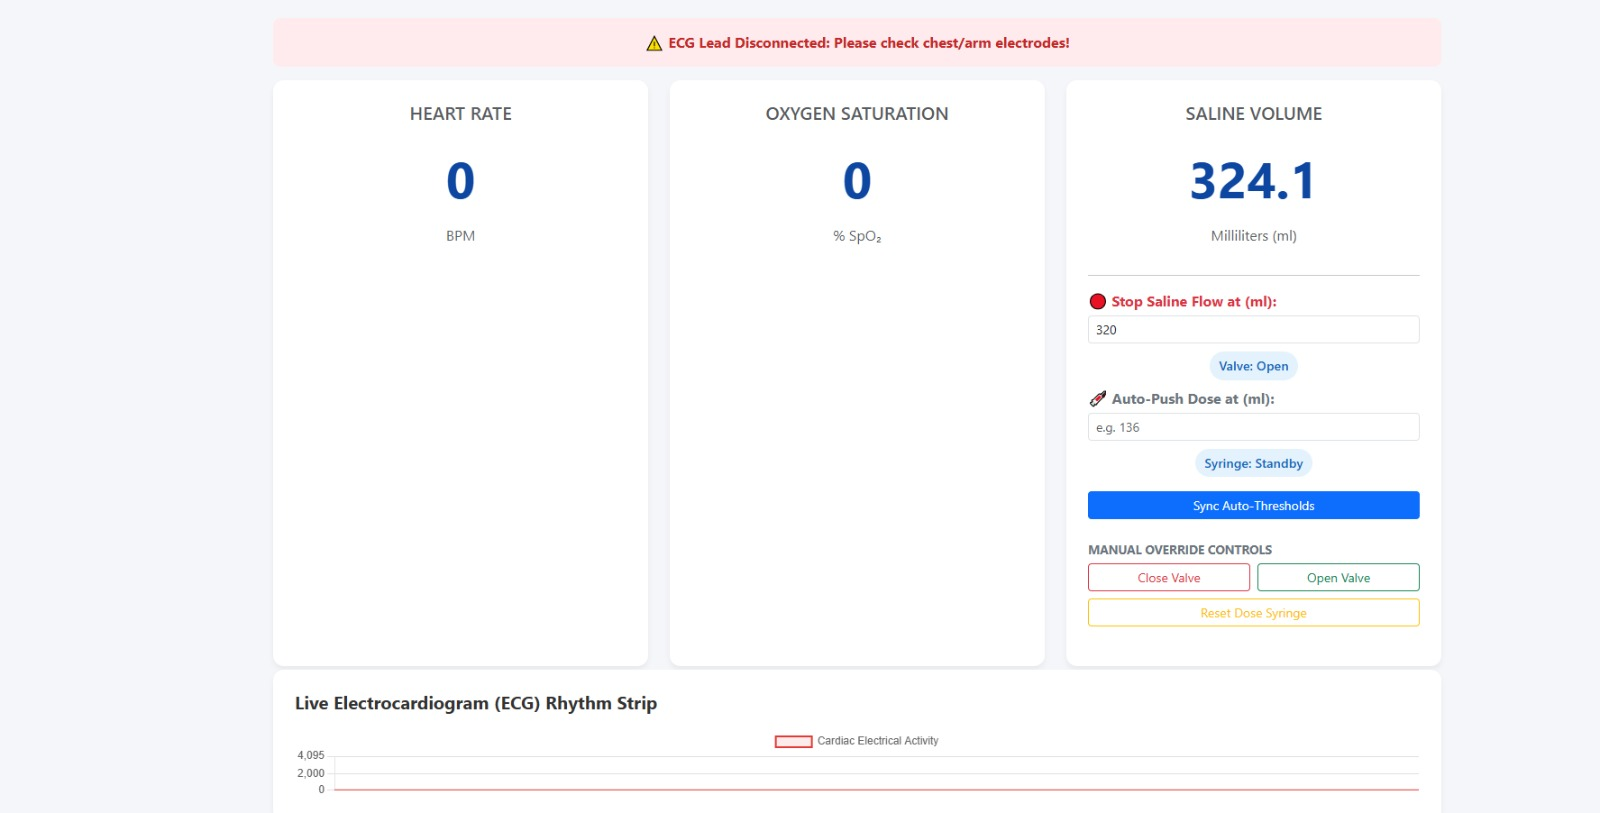
\includegraphics[width=0.97\textwidth]{web_1.jpeg}
\caption{Supplied doctor dashboard capture: estimated fluid 324.1~mL, configured stop threshold 320~mL, valve Open, syringe Standby, and unavailable physiological values. The zero ECG trace and disconnection banner document an interface state, without establishing a valid measured rhythm.}\label{fig:doctorresult}
\end{figure*}

Table~\ref{tab:observed} records the observation without assigning unmeasured performance values. The additional \code{saline_ml} and \code{saline_threshold} entries visible in the console screenshot are not read or written by the current active dashboard/firmware paths, and are not treated as the implemented data contract.

\begin{table}[!t]
\caption{Values Visible in the Supplied Captures}\label{tab:observed}
\centering\footnotesize
\begin{tabularx}{\columnwidth}{@{}P{0.31\columnwidth}P{0.20\columnwidth}Y@{}}
\toprule
Quantity & Visible value & Supported interpretation \\
\midrule
Fluid estimate & 324.1~mL & Displayed estimate; calibration unverified. \\
Saline stop setting & 320~mL & Positive remaining-volume cutoff. \\
Saline state & Open & Consistent with estimate above cutoff. \\
Dose trigger & 0 & Volume-trigger rule disabled in console snapshot. \\
Syringe state & Standby & No stroke shown at capture time. \\
Pulse / oxygen & 0 / 0 & Unavailable readings; no physiological accuracy evidence. \\
ECG & 0 & Doctor view shows disconnection warning and zero plot. \\
\bottomrule
\end{tabularx}
\end{table}

\subsection{Patient and Family Interface Outputs}
Fig.~\ref{fig:patientresult} shows the patient dashboard labeling the zero pulse and oxygen values as \emph{Sensor Ready / Place Finger}. Fig.~\ref{fig:familyresult} shows the corresponding family view. The family implementation excludes zero values from its positive-low-reading tests, so the lack of a family alarm in this capture is consistent with its code. It does not demonstrate that an abnormal valid measurement was detected or that a notification reached a caregiver.

\begin{figure}[!t]
\centering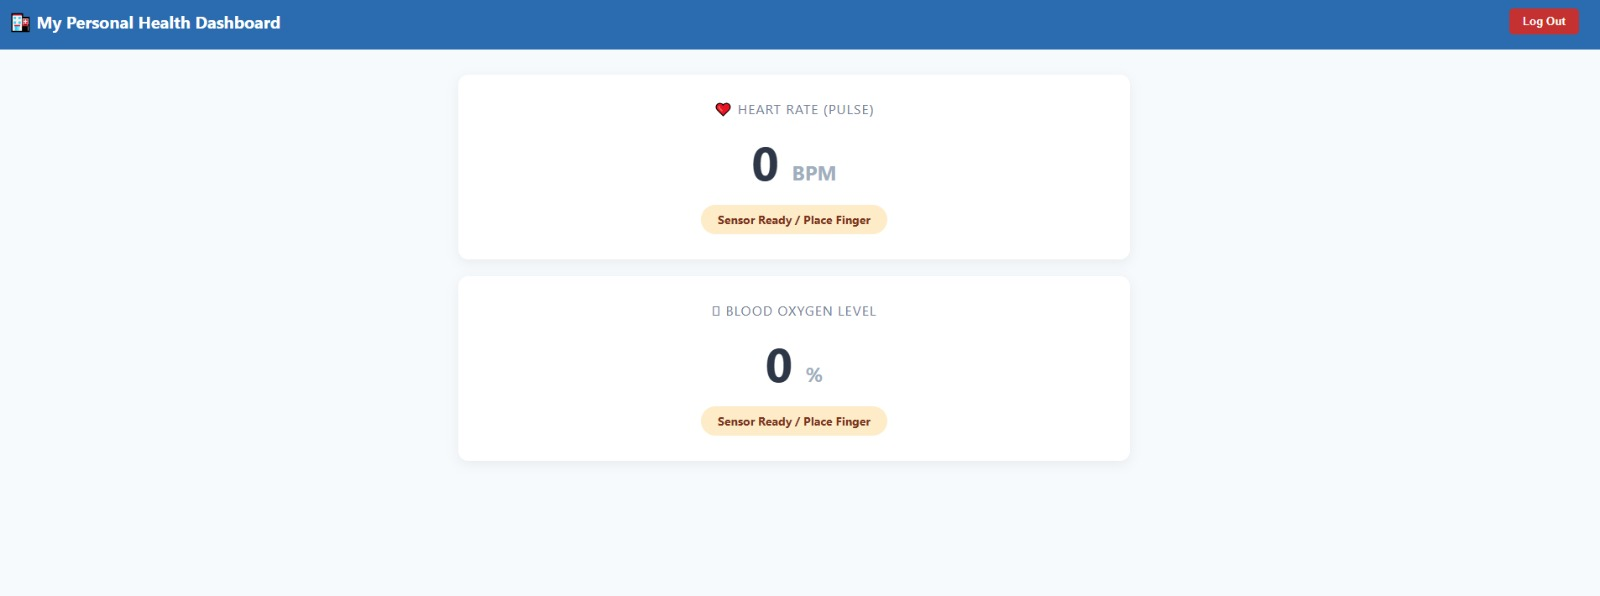
\includegraphics[width=\columnwidth]{web_5.jpeg}
\caption{Patient dashboard capture displaying zero readings and sensor-ready messages. The image demonstrates the unavailable-reading presentation rather than validated physiological sensing.}\label{fig:patientresult}
\end{figure}
\begin{figure}[!t]
\centering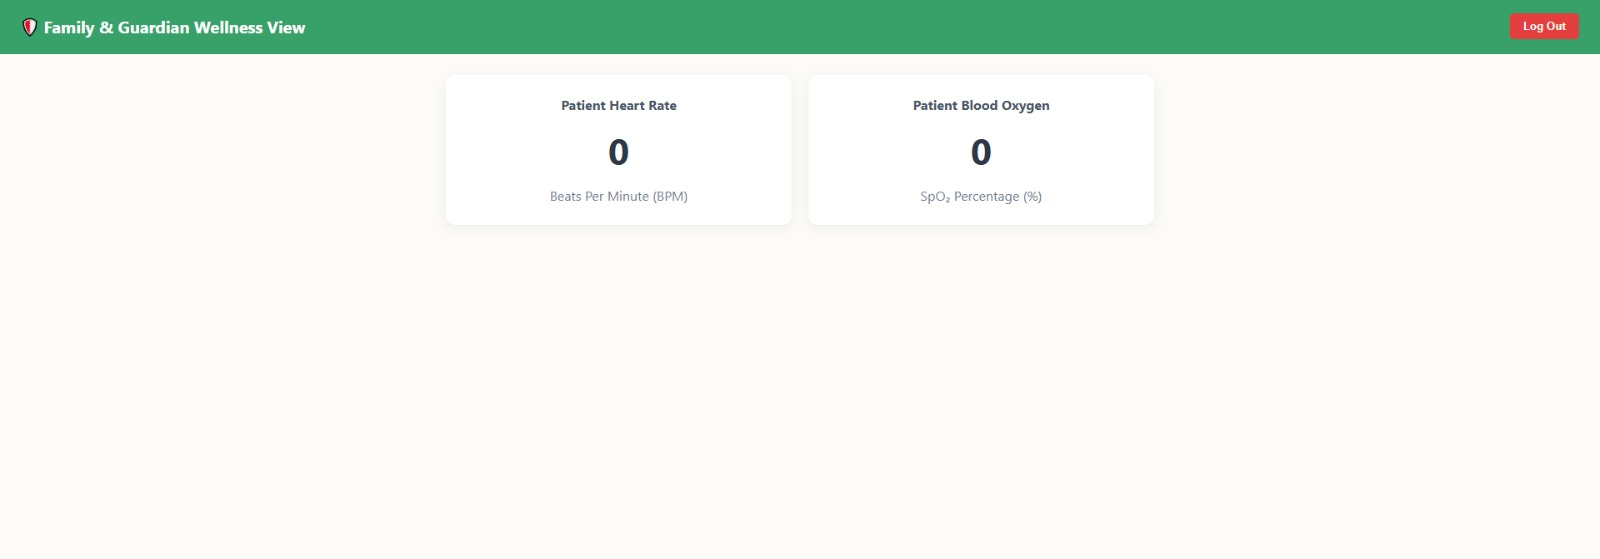
\includegraphics[width=\columnwidth]{web_2.jpeg}
\caption{Family/guardian dashboard capture. No alert is visible for the captured zero values, which the implemented alert condition excludes.}\label{fig:familyresult}
\end{figure}

The account-creation screenshot contains the patient, family/guardian, and medical-doctor role choices. Source inspection confirms the intended authentication and routing sequence. Successful registration of every role, enforcement of doctor privileges, and protected access to telemetry are not established by that single screenshot.

\subsection{Source-Derived Output Conditions}
The prototype's key output conditions are explicit in the firmware. The following excerpt is taken from the control-condition portion of \code{main.c}; it contains no credentials:
\begin{quote}\footnotesize
\begin{verbatim}
bool saline_stop_active =
  (saline_stop_ml > 0 &&
   current_ml < saline_stop_ml);
bool weight_trigger =
  (dose_trigger_ml > 0 &&
   current_ml < dose_trigger_ml);
bool o2_emergency =
  (smooth_spo2 > 0 &&
   smooth_spo2 < OXYGEN_DANGER_LEVEL);
\end{verbatim}
\end{quote}
When \code{o2_emergency} is true, the output branch calls \code{gpio_set_level(BUZZER_PIN, 1)} and advances the oxygen-designated servo angle. The code therefore establishes the command path from an estimated sensor value to a GPIO/PWM output. The supplied photographs do not capture the buzzer energized or provide measured oxygen flow, so physical alarm activation and treatment delivery are not reported as observed results.

Table~\ref{tab:logiccases} presents illustrative boundary cases derived from these conditions. These are analytic examples, not newly conducted bench tests or recorded patient data.
\begin{table*}[!t]
\caption{Illustrative Input-to-Output Cases Derived from the Firmware}\label{tab:logiccases}
\centering\small
\begin{tabularx}{\textwidth}{@{}P{0.21\textwidth}P{0.27\textwidth}YY@{}}
\toprule
Case & Assumed inputs & Programmed outcome & Evidence status \\
\midrule
Captured saline state & $V=324.1$~mL, $T_s=320$~mL & Closing condition false; target moves toward open. & Values/status visible in saved captures and consistent with code. \\
Saline threshold equality & $V=320$~mL, $T_s=320$~mL & Strict comparison false; does not begin closing. & Boundary example from source only. \\
Below saline cutoff & $V=319$~mL, $T_s=320$~mL & Servo moves toward clamp; Closing then Stopped if condition persists. & Source-derived case; no matching observed sequence supplied. \\
Volume-triggered syringe & $V=135$~mL, $T_d=136$~mL; cycle inactive & Begins fixed forward/return angle sequence. & Source-derived case; delivered volume unmeasured. \\
Low estimated oxygen & $S=84\%$ with usable optical input & Buzzer GPIO high; oxygen-designated servo advances. & Source-derived case; alarm/flow not experimentally documented. \\
Unavailable optical input & Infrared count below 20000 & Pulse and oxygen estimates zero; positive-low-oxygen condition false. & Source branch; zero outputs are visible, but raw optical input was not recorded. \\
ECG lead off & LO+ or LO$-$ high & ECG value forced to zero; doctor page shows warning. & Source branch; warning visible, input-pin state unrecorded. \\
\bottomrule
\end{tabularx}
\end{table*}

\subsection{Timing and Efficiency That Can Be Inferred}
The 20~ms programmed loop delay and angular increments yield nominal delay-only travel times: $90\times20$~ms $=1.8$~s for a $180^{\circ}$ saline/oxygen command, $180\times20$~ms $=3.6$~s for the syringe's forward stroke, and about 1.8~s for its return. Sensor access and transition iterations add time, and mechanical motion may differ from the command sequence. These values are calculations from the implementation, not measured response times.

The cloud task delays two seconds after completing its requests, so it offers periodic latest-value publication with additional HTTP overhead. The doctor plot appends one ECG value per database callback rather than a timestamped waveform packet. Consequently, the captured flat plot and software timing do not establish ECG waveform fidelity. No current measurements, battery-capacity specification, deployment uptime, or itemized purchase costs are provided, so energy efficiency, battery life, and total cost remain unquantified.

\subsection{Experimental Validation Required for Performance Claims}
Table~\ref{tab:validation} specifies the missing measurements and an appropriate way to obtain them. These procedures are proposed future evaluation, not completed experiments. Fluid and syringe trials should use a laboratory collection setup; any human physiological study requires the relevant supervision and consent arrangements.

\begin{table*}[!t]
\caption{Proposed Validation Plan; No Results Are Claimed for These Tests}\label{tab:validation}
\centering\small
\begin{tabularx}{\textwidth}{@{}P{0.20\textwidth}YY@{}}
\toprule
Subsystem & Proposed procedure & Record and evaluation metric \\
\midrule
Fluid estimate & Tare the empty assembly; apply known loads/volumes across its range; repeat static and disturbed trials. & Reference/estimated volume pairs; mean absolute error, maximum error, repeatability, and mounting conditions. \\
Saline stopping & Move the measured estimate through positive thresholds, equality, and disabled settings; collect remaining leakage after closure. & Input, GPIO/PWM time, physical closure time, state sequence, and residual fluid movement. \\
Syringe mechanism & Calibrate syringe geometry/travel using collected fluid; repeat full-stroke trials under specified loads. & Reference delivered volume, variation, backlash, stalls, and mechanical limits. \\
Pulse / SpO\textsubscript{2} & Compare synchronized valid outputs with an appropriate reference instrument and document signal/motion conditions. & Paired readings, acquisition availability, agreement errors, and recovery after signal loss. \\
ECG channel & Use a known simulator/reference signal and record locally timestamped samples; exercise both lead-off inputs. & Sampling interval/jitter, signal agreement, lead-off detection, and cloud information loss. \\
Cloud/control & Timestamp a setting change, device receipt, output command, and browser status; repeat with delays/disconnection. & Median/maximum end-to-end times, failed writes, stale-data behavior, and recovery. \\
Power and operation & Measure voltage/current with Wi-Fi and servos active, and observe resets/stalls on the actual supply. & Peak current, energy per interval, operating duration, and brownout behavior. \\
\bottomrule
\end{tabularx}
\end{table*}

For $N$ paired reference and estimated volumes, a reproducible accuracy summary would include
\begin{equation}
\mathrm{MAE}_V=\frac{1}{N}\sum_{i=1}^{N}|\hat V_i-V_i^{\mathrm{ref}}|\quad(\mathrm{mL}).
\end{equation}
An end-to-end control measurement would separately record database write time, device receipt time, and physical actuator response. No values for these metrics are inserted because the required paired records and timestamps are absent.

